\documentclass{foi}
\usepackage[utf8]{inputenc}
\usepackage{lipsum}

\vrstaRada{\zavrsni} % \diplomski
\title{Dodavanje funkcionalnosti u jezgru operacijskoga sustava TempleOS}

\author{Viktor-Alojzije Ćorić}
\spolStudenta{\musko} % \zensko ili \musko
\mentor{Luka Milić}
\spolMentora{\musko} % \zensko ili \musko
\godina{2021}
\mjesec{rujan}
\date{2021}
%\status{redoviti}
\indeks{0016140113}
\smjer{Informacijski sustavi} % (ili Poslovni sustavi, Ekonomika poduzetništva, Primjena informacijske tehnologije u poslovanju, Informacijsko i programsko inženjerstvo, Baze podataka i baze znanja, Organizacija poslovnih sustava, Informatika u obrazovanju)
\titulaProfesora{mag. ing. comp.}

\sazetak{TempleOS je besplatni 64-bitni operacijski sustav u javnoj domeni. Operacijski sustav je pisan iz temelja, a sve napisano je djelo jednoga čovjeka koji je patio od shizofrenije, Terrya A. Davisa. Unutar samoga operacijskoga sustava postoji puno novotarija, kao što su vlastiti kompilator, vlastiti programski jezik, vlastiti format za dokumente, vlastiti datotečni sustav, vlastite grafičke knjižnice pisane iz temelja, itd. Cijeli operacijski sustav radi u načinu rada \emph{Ring 0}, te je stoga zanimljivo promatrati ga iz programerskoga pogleda. U radu se objašnjavaju osnove operacijskoga sustava, najzanimljivije značajke, dodavanje funkcionalnosti u korisnički prostor, dodavanje funkcionalnosti u jezgru, koje će se demonstrirati u vidu dodavanja hrvatskih znakova i tipkovnice, te kako preinačenu inačicu sustava dalje distribuirati.}

\kljucneRijeci{TempleOS, jezgra, operacijski sustavi, tipkovnica, znakovi}

\begin{document}

\maketitle

\tableofcontents

\pagestyle{plain}
\chapter{Uvod}

TempleOS je besplatni 64-bitni operacijski sustav koji je u javnoj domeni. Autor operacijskoga sustava je američki programer Terry A. Davis, koji je sam izradio svaku sastavnicu operacijskoga sustava, od programskoga prevoditelja do slikovnih elemenata, kao i programski jezik HolyC, datotečni sustav RedSea, i sl.

Pripovijest iza samoga operacijskoga sustava je zanimljiv dio vrijedan spomena. Naime, Terry A. Davis je za vrijeme svoga života patio od shizofrenije, i često je imao deluzije različitih sadržaja, od zamišljenih prijatelja s kojima je razgovarao do agenata američke Središnje Obavještajne Agencije koji su ga pratili. U jednoj od takvih epizoda, navodno, ukazao mu se je i sam Bog, koji je htio da mu Davis izgradi Treći Hram. Bog mu je isto tako, navodno, dao i precizne specifikacije operacijskoga sustava: razlučivost 640x480, 16-bitne boje, jednokanalni audio sustav, itd. Vjerska tematika operacijskoga sustava mogla je se naslutiti iz već spomenutih HolyC (Holy See – Sveta Stolica), RedSea (Crveno more), iz samoga naziva TempleOS (Temple – Hram), ali i iz sastavnica koje će se poslije spomenuti (Adam npr.).

Operacijski sustav sveukupno sadržava 119667 redaka koda, koji uključuju jezgru operacijskoga sustava, 64-bitni programski prevoditelj, grafičke knjižnice i sva potrebna oruđa za rad sa sustavom \cite{TOS}. Jedan od ciljeva operacijskoga sustava je i da smanji broj redaka koje sami programer-korisnik mora rabiti, tako da bi se napisao program \emph{hello world} u HolyC-u, potrebno je samo napisati {\fontfamily{pcr}\selectfont "Hello World";}, a složenost se može povećavati ovisno o potrebama korisnika, mogu se dodavati funkcije kao u programskom jeziku C (gdje je za razliku od HolyC-a funkcija \emph{main} obvezna), te se može pisati i u zbirnom jeziku.

TempleOS sve operacije obavlja u načinu rada \emph{Ring 0}, što znači da korisnik ima pristup svemu i da nema zaštite memorije. Bilo kako bilo, jedno ponovno pokretanje računala rješava većinu problema vezanih za memoriju, kao što se je i autor sam uvjerio prigodom izradbe završnoga rada.

O potankostima operacijskoga sustava više u nadolazećim poglavljima, kao i o projektnom zadatku, koji je bio izradba tipkovnice na hrvatskom jeziku.

\chapter{Operacijski sustav TempleOS}

U ovom poglavlju će se objasniti proces instalacije operacijskoga sustava, objasniti kako se operacijski sustav rabi, te opisati najzanimljivije značajke operacijskoga sustava.

\section{Instalacija TempleOS-a\label{instalacijaTOSa}}

ISO-slika operacijskoga sustava TempleOS se može preuzeti na poveznici \url{https://templeos.org}, gdje se preuzima {\fontfamily{pcr}\selectfont TempleOS.ISO} ili {\fontfamily{pcr}\selectfont TempleOSLite.ISO}. Nema nekoga posebnoga razloga zašto rabiti inačicu Lite, jer je puna inačica 17 MB, tako da s inačicom Lite se štedi 15 MB memorijskoga prostora, što je zanemarivo. Isto tako postoje i dopunske ISO-slike, koje sadržavaju neke dodatne stvari, kao npr. videoigru AfterEgypt, koja se ne nalazi u datoteci {\fontfamily{pcr}\selectfont TempleOS.ISO}. Dopunske datoteke se montiraju unutar sustava.

TempleOS radi na virtualnim strojevima VMWare, QEMU i VirtualBox. Autor operacijskoga sustava je rabio virtualni stroj VMWare, dok je prigodom izradbe ovoga rada rabljen virtualni stroj QEMU s modulom KVM.

Instalacija je prilično jednostavna, treba se pritisnuti {\fontfamily{pcr}\selectfont y} za instalaciju na tvrdi disk, za odabir se pritišće {\fontfamily{pcr}\selectfont y} ako se rabi virtualni stroj, pritišće se bilo koja tipka, čeka se približno jednu minutu da se instalacija dovrši, te se pritišće {\fontfamily{pcr}\selectfont y} za ponovno pokretanje. Nakon toga je cijeli operacijski sustav instaliran. Prigodom prvoga pokretanja treba pričekati par sekundâ da se dekomprimiraju pojedine datoteke, i nakon toga je operacijski sustav spreman za rad. Opcionalno se nudi vodič za porabu sustava.

\section{Poraba TempleOS-a}

Dio koji najviše zbunjuje korisnika prigodom prvoga pokretanja TempleOS-a je korisničko sučelje. Navigirati je moguće pomoću miša, ali i samo pomoću tipkovnice, pomoću strjelica, tipke {\fontfamily{pcr}\selectfont SPACE} (lijevi pritisak tipke na mišu) i tipke {\fontfamily{pcr}\selectfont ENTER} (desni pritisak tipke na mišu). U zadanom sučelju se nalaze dva otvorena prozora, a preko desnoga prozora se može vidjeti i mali sivi prozorčić koji služi kao \emph{autocomplete}, i on korisniku izbacuje moguće prijedloge za automatsko nadopunjanje, a korisnik nadopunja započetu riječ pomoću tipke {\fontfamily{pcr}\selectfont CTRL} u kombinaciji s tipkom koja stoji uz predloženu riječ.

Da bi se za početak korisnik lakše snašao, preporuka je zatvoriti jedan prozor pritiskom na {\fontfamily{pcr}\selectfont X} u gornjem desnom kutu, ili pritiskom tipaka {\fontfamily{pcr}\selectfont SHIFT-ESC}, te drugi prozor proširiti povlačenjem njegova ruba mišem.

Pritiskom na tipke {\fontfamily{pcr}\selectfont CTRL-M} otvara se interaktivni izbornik u kojem se korisnik može dalje upoznati s operacijskim sustavom, ali i u kojem može pokretati videoigre koje je autor Terry Davis sam izradio. Iz izbornika se izlazi na tipku {\fontfamily{pcr}\selectfont ESC}.

Kroz kazala korisnik se navigira ili grafičkim putem (miš ili tipkovnica), ili kroz naredbeni redak preko naredbe {\fontfamily{pcr}\selectfont Cd;}. Sve što se upiše u naredbeni redak izravno ide u kompilator i tu se obrađuje, to je tzv. kompilacija JIT.

Budući da privlačnost TempleOS-a ne leži u onom što operacijski sustav već nudi, već u onom što se može s njim raditi, TempleOS je ipak privlačniji programerima i hobistima nego osobama koje se bave uredskim poslovima. Stoga, to bi bilo to što se tiče „korisničkog” dijela, a u sljedećem poglavlju će se opisati naprjednija poraba kroz programiranje.

\section{Programiranje u TempleOS-u / HolyC-u}

HolyC je programski jezik koji se rabi u TempleOS-u, a kompilatori za HolyC na ostalim operacijskim sustavima (koji nisu derivati TempleOS-a) ne postoje. Jezik je osmišljen da bude što jednostavniji, slično kao i programski jezik BASIC.

Programski jezik HolyC poznaje sljedeće vrste podataka: {\fontfamily{pcr}\selectfont U0}, {\fontfamily{pcr}\selectfont U8}, {\fontfamily{pcr}\selectfont U16}, {\fontfamily{pcr}\selectfont U32} i {\fontfamily{pcr}\selectfont U64} za nepredznačene cijele brojeve veličina 0, 1, 2, 4 i 8 bajtova, {\fontfamily{pcr}\selectfont I0}, {\fontfamily{pcr}\selectfont I8}, {\fontfamily{pcr}\selectfont I16}, {\fontfamily{pcr}\selectfont I32} i {\fontfamily{pcr}\selectfont I64} za predznačene cijele brojeve veličina 0, 1, 2, 4 i 8 bajtova. Također postoji i {\fontfamily{pcr}\selectfont F64}, koja stoji za tip podataka \emph{float} veličine 8 bajtova. Tipovi podataka za 32-bitni \emph{float} ne postoje.\cite{HolyC}

Programski jezik podupire sve petlje kao i u programskom jeziku C (\emph{for}, \emph{while} i \emph{do-while}), dok je uvjetna naredba \emph{if} nešto naprjednija u usporedbi sa svojim C i C++ protulikovima (izraz {\fontfamily{pcr}\selectfont 5 < i <= j + 1 < 20} je u potpunosti validan izraz, dok bi se kod C/C++-a trebalo tipkati {\fontfamily{pcr}\selectfont 5 < i \&\& i <= j + 1 \&\& j + 1 < 20}) \cite{HolyC}.

Na konkretnom primjeru iz Sl. \ref{fig:helloworld} će se objasniti osnove programskoga jezika HolyC, a zatim će se spomenuti i naprjednije potankosti.

\begin{figure}[H]
    \centering
    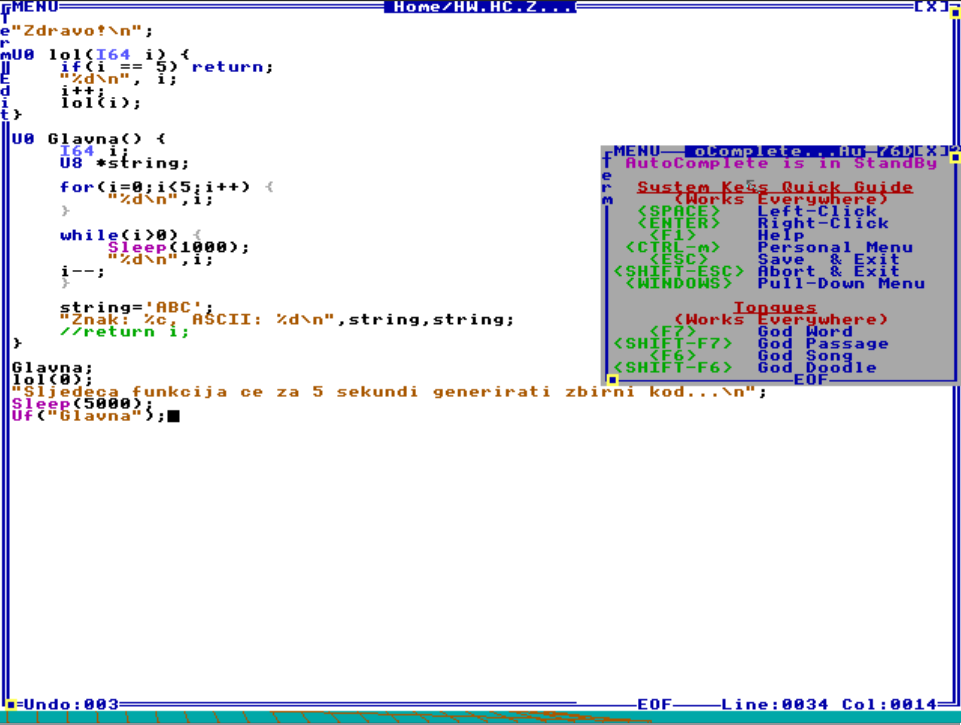
\includegraphics[width=1.0\textwidth]{slike/helloworld.png}
    \caption{Primjer programa u jeziku HolyC}
    \label{fig:helloworld}
\end{figure}

\begin{itemize}
    \item Prvi redak jednostavno ispisuje {\fontfamily{pcr}\selectfont Zdravo!} na zaslon.

    \item Deklarira se funkcija {\fontfamily{pcr}\selectfont lol}, koja je zamišljena kao rekurzivna funkcija. Odbrojava do 5 sve dok ne dođe do sidrenoga uvjeta (engl. \emph{anchor case}).

    \item U funkciji {\fontfamily{pcr}\selectfont Glavna} se pokazuje kako se deklariraju cijeli 64-bitni brojevi, te kako se deklarira pokazivač. Nakon deklaracije se pokazuje rad s petljama, petlja \emph{for} odbrojava od {\fontfamily{pcr}\selectfont 0} do {\fontfamily{pcr}\selectfont 4}, dok petlja \emph{while} odbrojava od {\fontfamily{pcr}\selectfont 5} do {\fontfamily{pcr}\selectfont 1} (tu se još demonstrira i funkcija {\fontfamily{pcr}\selectfont Sleep}). Nakon toga se inicijalizira znakovni niz, i ispisuje se njegova stvarna i brojčana vrijednost. Funkcija može i vraćati određene podatke.

    \item Nakon deklaracije funkcije {\fontfamily{pcr}\selectfont Glavna} dolazi pozivanje tih funkcija. Kao što se vidi, funkcija {\fontfamily{pcr}\selectfont lol} prima jedan parametar. Funkcija {\fontfamily{pcr}\selectfont Glavna} se može pozivati sa zagradama i bez njih.

    \item Funkcija {\fontfamily{pcr}\selectfont Uf} obilježava {\fontfamily{pcr}\selectfont Unassemble function}, te vraća kod rečene funkcije u zbirnom jeziku.
\end{itemize}

HolyC isto tako podupire i koncepte unija i razreda. Unija djeluje na isti način kako i djeluje u C/C++-u, dok je koncept razreda ostvaren kao nešto između C/C++-ovoga {\fontfamily{pcr}\selectfont structa} i C++-ova razreda, jer postoji i svojstvo nasljeđivanja povrh običnoga {\fontfamily{pcr}\selectfont structa}.

Postoje dvije vrste kompilacije u TempleOS-u, a to su Just In Time (JIT) i Ahead Of Time (AOT). Kompilacija JIT se rabi za veliku većinu svih radnjâ u operacijskom sustavu, jedini dio koda koji se prevodi Ahead of Time (AOT) je jezgra operacijskoga sustava, za koju se prigodom prevođenja stvara binarna datoteka. Kompilacija JIT omogućuje da se HolyC rabi i kao naredbeni redak tj. ljuska operacijskoga sustava. Svaka naredba koja se upiše izravno ide u programski prevoditelj. Razlog toga je što autor operacijskoga sustava nije bio ljubitelj razlikovanja između sintakse programskih jezika (C, C++) i naredaba za upravljanje operacijskim sustavom ({\fontfamily{pcr}\selectfont bash}).

Neke zanimljivosti i novosti u programskom jeziku HolyC su:
\begin{itemize}
    \item Funkcije bez argumenata ne trebaju zagrade.

    \item Argumenti sa zadanim vrijednostima ne moraju se deklarirati na kraju.

    \item Uvjeti se mogu staviti pod jedan izraz, npr. {\fontfamily{pcr}\selectfont 5 <= x < y < 15 == z}, umjesto 4 izraza koja bi kombinirali s operatorom {\fontfamily{pcr}\selectfont \&\&} u C-u i C++-u \cite{HolyC}.

    \item \emph{Switch} može imati i pod-\emph{switch}, \emph{switch} unutar \emph{switcha}, rabeći ključne riječi \emph{start} i \emph{end} \cite{HolyC}.

    \item {\fontfamily{pcr}\selectfont U0} tip podatka, koji je jednakovrijednica tipu podatka {\fontfamily{pcr}\selectfont void} u C-u i C++-u zauzima 0 bajtova, za razliku od {\fontfamily{pcr}\selectfont voida} u GNU-ovu dijalektu C-a koji zapravo zauzima jedan bajt.

    \item Funkcije imaju ugrađene varijable za brojenje argumenata i čitanje istih ({\fontfamily{pcr}\selectfont argc} i {\fontfamily{pcr}\selectfont argv}), te djeluju na sličan način kao što djeluje operator \emph{this} u jeziku C++ \cite{HolyC}.

    \item HolyC ima potporu za \emph{try-catch-throw}.

    \item Direktiva {\fontfamily{pcr}\selectfont \#exe}, koja omogućuje izvršavanje naredbe i pohranjivanje njezine vraćene vrijednosti unutar programskoga koda.

    \item Sve vrijednosti se proširuju u 64 bita kada im se pristupa \cite{HolyC}.

\end{itemize}

\section{DolDoc}

DolDoc je TempleOS-ova vrsta dokumenta. Ono što je vrlo zanimljivo je da su svi izbornici koje korisnik vidi pisani u obličju DolDoc, a u to se može i uvjeriti pritiskom {\fontfamily{pcr}\selectfont CTRL+T} tipaka, koje će prebacivati između čistoga teksta i teksta s grafikama.

Ono što je specifično za obličje DolDoc je što se pored izvornoga koda programa TempleOS u nj mogu pohranjivati i 3D grafike, slike, itd., i program će se i dalje uspješno prevoditi i pokretati. Usporednica tomu bi bila kada bi se LibreOffice ili Microsoft Word rabio kao razvojna okolina.

Sve naredbe u DolDocu se moraju opkoliti znakom dolara, dakle primjer takve naredbe bi bio {\fontfamily{pcr}\selectfont \$CL\$}, naredba za brisanje zaslona koja je dosta slična funkciji {\fontfamily{pcr}\selectfont DocClear}, čija bi jednakovrijednica za Microsoft Windows bila {\fontfamily{pcr}\selectfont cls}, a jednakovrijednica za UNIX bila {\fontfamily{pcr}\selectfont clear}.

Naredaba ima previše, pa da se ne navode sve u radu, ako čitatelja zanima može ih pregledati u samom TempleOS-u pod {\fontfamily{pcr}\selectfont /Doc/DolDocOverview.DD.Z} (preporučljivo zbog organiziranosti), ili na referenciji \cite{DolDoc}.

\begin{figure}[H]
    \centering
    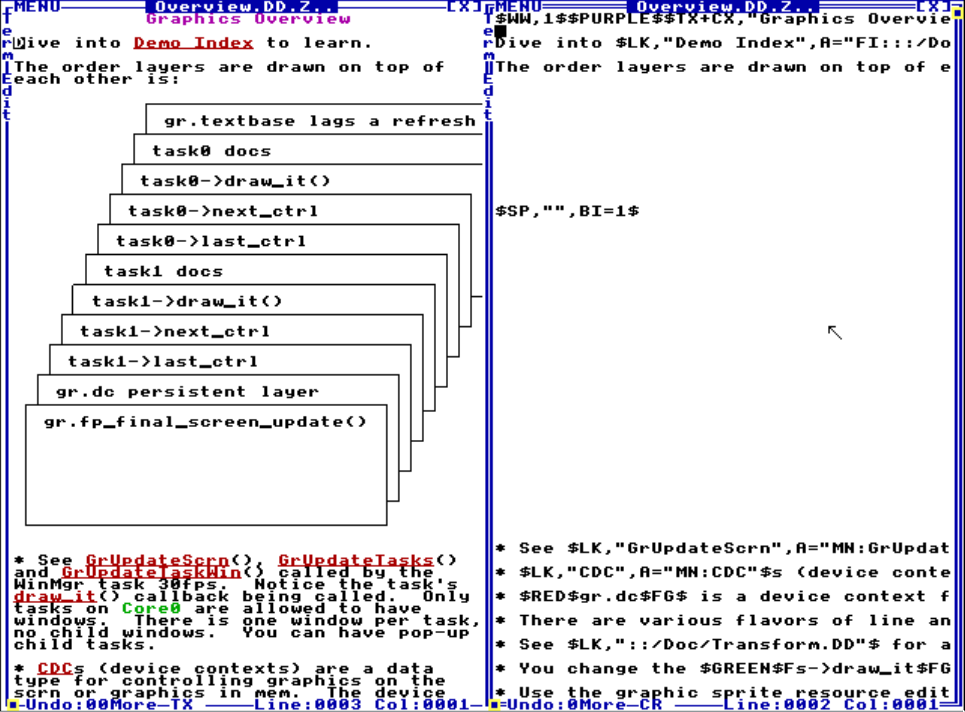
\includegraphics[width=1.0\textwidth]{slike/doldoc.png}
	\captionsetup{justification=centering}
    \caption{Primjer dokumenta DolDoc, na lijevoj slici je prikazan normalni prikaz, na desnoj slici je prikazan tekstualni prikaz}
    \label{fig:doldoc}
\end{figure}

\section{RedSea}

RedSea je datotečni sustav koji je Terry A. Davis napisao. TempleOS pored RedSea podupire i datotečne sustave FAT32 i ISO9660.

RedSea je jednostavni 64-bitni datotečni sustav koji je sličan datotečnom sustavu FAT32, ali umjesto grozdova rabi apsolutne blokove. FAT (\emph{File Allocation Table}) tablica nije implementirana jer je patentirana, te umjesto nje se rabi alokacijska bitmapa \cite{RedSea}.

Glavna prednost datotečnoga sustava RedSea je jednostavnost. Autor TempleOS-a često navodi Commodore 64 kao svoju nadahnutost za većinu toga u operacijskom sustavu, te datotečni sustav RedSea tu nije iznimka. Autor se je dojmio kako je korisnik Commodorea 64 mogao izravno pristupiti diskovnim blokovima i kako je mogao povratiti obrisane datoteke iz tih blokova.

RedSea rabi alokacijsku bitmapu susjednih datoteka, ne prati pokvarene blokove i zalihosne FAT-ove. Susjedna alokacija je iznimno jednostavna i brza, ali nije toliko efikasna jer je takav datotečni sustav skloniji fragmentaciji i dosta se prostora troši nepotrebno \cite{tannenbaum1997}. Kod TempleOS-a to nije problem doduše jer je sam autor zabranio da se rabe multimedijske datoteke \cite{BlockChain} \cite{RedSeaReliablility}, navodeći fragmentaciju memorije kao ozbiljan problem.

Još jedna zanimljiva značajka datotečnoga sustava RedSea je što on sam komprimira sve datoteke koje završavaju proširkom {\fontfamily{pcr}\selectfont .Z}. \cite{BlockChain} Kada se pokuša otvoriti datoteka koja završava s proširkom {\fontfamily{pcr}\selectfont .Z}, uređivač teksta \emph{vim} javlja pogrješku da se radi o komprimiranoj datoteci, iako je dio teksta donekle čitljiv.

Sada kada su spomenute i opisane najzanimljivije značajke TempleOS-a, može se početi s opisivanjem praktičnoga dijela ovoga rada.

\chapter{Dodavanje funkcionalnosti u TempleOS}

Funkcionalnosti se u operacijski sustav TempleOS mogu dodavati na dva načina, unutar korisničkog prostora, koje se može obavljati na dva načina, i unutar jezgre.

Treba voditi računa da se funkcionalnosti u korisničkom prostoru prevode Just In Time (JIT), dok se funkcionalnosti u jezgri prevode Ahead Of Time (AOT).

\section{Dodavanje funkcionalnosti u korisnički prostor}

Dodavanje funkcionalnosti u korisnički prostor unutar TempleOS-a je jednostavno kao i na bilo kojem drugom operacijskom sustavu, jedina razlika dodavanja funkcionalnosti u Temple\-OS-u je to što od razvojnih oruđa ima dostupne samo zbirni jezik i programski jezik HolyC za programiranje, dok u drugim operacijskim sustavima većinom ima širi spektar razvojnih alata.

Za dodavanje funkcionalnosti u korisnički prostor je potrebno prvo napisati željeni program. Primjer koji će biti prikazan u svrhu prikaza dodavanja programa je primjer sa Sl. \ref{fig:helloworld}.

Postoji više načina kako dodati funkcionalnost u korisnički prostor operacijskog sustava TempleOS, a to su:

\begin{itemize}
    \item Otvaranje datoteke u uređivaču teksta i pritisak tipke {\fontfamily{pcr}\selectfont F5}.
    \item Pokretanje pomoću direktive {\fontfamily{pcr}\selectfont \#include}.

    \item Pokretanje programa tijekom prevođenja nekog drugog programa pomoću direktive {\fontfamily{pcr}\selectfont \#exe}.

    \item Pokretanje datoteke unutar Adama (trajni kod).
\end{itemize}

Pokretanje pomoću tipke {\fontfamily{pcr}\selectfont F5} unutar uređivača teksta je jasna sama po sebi, potrebno je otvoriti željenu datoteku i pritisnuti {\fontfamily{pcr}\selectfont F5}.

Pokretanje pomoću direktive {\fontfamily{pcr}\selectfont \#include} se vrši tako što unutar ljuske operacijskoga sustava se piše naredba {\fontfamily{pcr}\selectfont \#include "<naziv datoteke bez proširke>";}. Isto tako, budući da sve naredbe iz ljuske idu izravno u kompilator i prevode se Just In Time (JIT), ovakav način pokretanja programa se može rabiti i unutar drugoga programa.

Operacijski sustav TempleOS nudi i jednu zanimljivu značajku, a to je direktiva {\fontfamily{pcr}\selectfont \#exe}, koja omogućuje izvršavanje koda tijekom procesa prevođenja, te se taj kod može umetnuti u tok koji se prevodi \cite{PreProcessor}. To je HolyC-ova alternativa za makronaredbe znane iz programskih jezika C/C++.

Dodavanje funkcionalnosti u korisnički prostor se može odraditi na još jedan način, koji je više križanac između korisničkog i sustavskog prostora, a to je pomoću Adama, koji je prvi proces koji se stvara i koji se ne može ugasiti.

\begin{figure}[H]
    \centering
    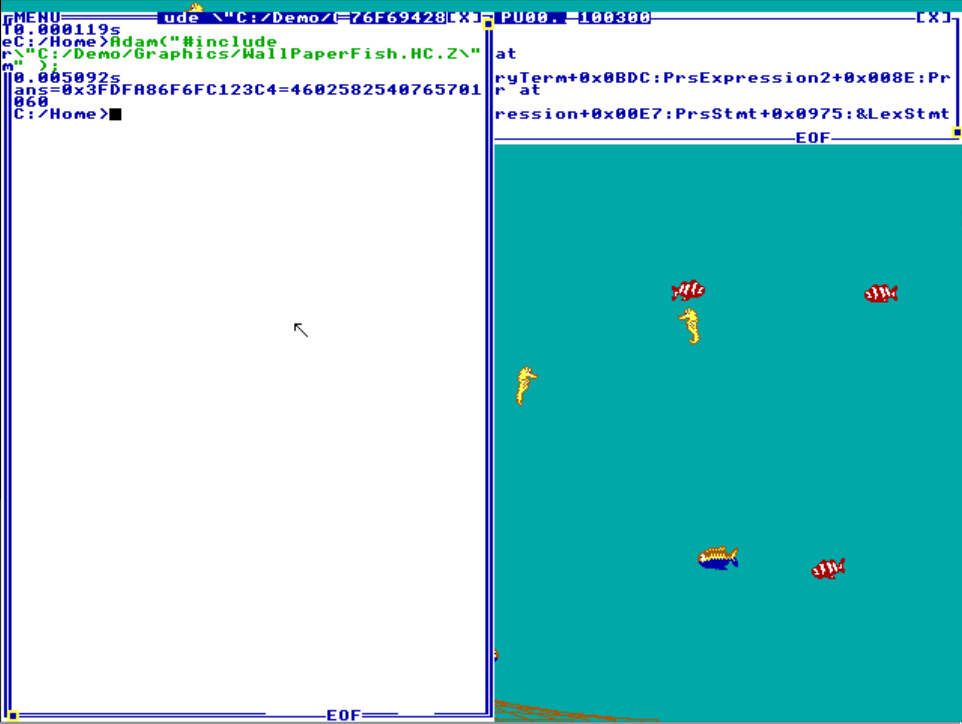
\includegraphics[width=1.0\textwidth]{slike/adamwp.png}
	\caption{Program uključen preko Adama, postavlja dinamičku pozadinu koja se miče}
    \label{fig:adamwp}
\end{figure}

\section{Dodavanje funkcionalnosti u jezgru}

Dodavanje funkcionalnosti u jezgru je nešto zahtjevniji zadatak, ali opet je puno jednostavnije u usporedbi s drugim operacijskim sustavima.

Prigodom dodavanja funkcionalnosti u jezgru operacijskoga sustava TempleOS treba voditi računa da je jezgra jedini dio TempleOS-a koji se prevodi Ahead Of Time (AOT), te da se sve operacije unutar jezgre uvode u načinu rada kojeg autor operacijskoga sustava naziva \emph{raw mode}. Programiranje je drugačije nego u korisničkom prostoru jer se nema fleksibilnost koju nudi način prevođenja Just In Time. Primjerice, kada bi se deklarirala funkcija koja se izvršava u jezgri koja bi na pritisak tipke izvršila neki program unutar korisničkog prostora, prigodom prevođenja jezgre bi se dogodila pogrješka, jer se ne bi moglo pozicionirati na odgovarajuću lokaciju da bi se izvršila rečena datoteka, jer jezgra nema predznanje o ostalim dijelovima koda koji se ne prevode načinom AOT.

Kao što je već spomenuto u odlomku iznad, sav napisani kod u jezgrenom prostoru potrebno je prevesti načinom AOT. To se postiže pomoću funkcije {\fontfamily{pcr}\selectfont BootHDIns;}, koja će se potanje objasniti u nastavku.

\begin{figure}[H]
    \centering
    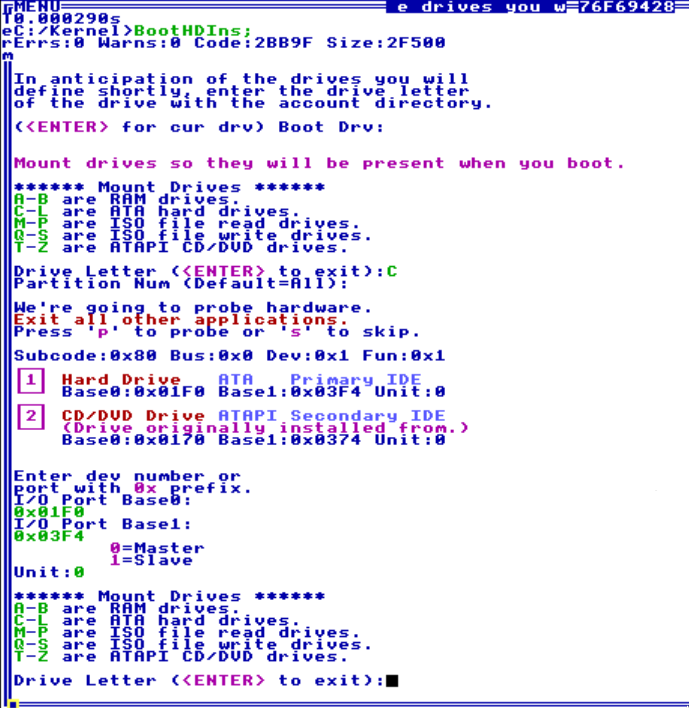
\includegraphics[width=1.0\textwidth]{slike/kernelcomp1.png}
	\caption{Prevođenje jezgre – osnovne postavke}
    \label{fig:kernelcomp1}
\end{figure}

Kao što je vidljivo na Sl. \ref{fig:kernelcomp1} i \ref{fig:kernelcomp2}, za prevođenje jezgre su za neke stvari dovoljne postavke, ali ipak je potrebna i određena količina ljudskog međudjelovanja za uspješno prevođenje. Ono što korisnik treba u velikoj većini slučajeva učiniti jest odabrati disk čija se jezgra prevodi, a to su većinom diskovi {\fontfamily{pcr}\selectfont C} i {\fontfamily{pcr}\selectfont D}, ovisno o tom što je odabrano prigodom dizanja operacijskoga sustava. Zatim je potrebno pritisnuti tipku {\fontfamily{pcr}\selectfont p} da bi saznale informacije o trenutnom disku, te iz tih informacija potrebno je ili pritisnuti broj koji se nalazi lijevo od diska, ili ručno upisati podatke o disku, odnosno njegov \emph{Base0}, \emph{Base1}, te \emph{Unit}. U primjeru na Sl. \ref{fig:kernelcomp1} odlučeno je ručno upisati podatke o disku. U primjeru na Sl. \ref{fig:kernelcomp2} su prikazane naprjednije opcije dostupne prigodom prevođenja jezgre, ali su one ostavljene na zadanim vrijednostima, a slika je uključena samo da bi se prikazalo koje su to naprjednije postavke.


\begin{figure}[H]
    \centering
    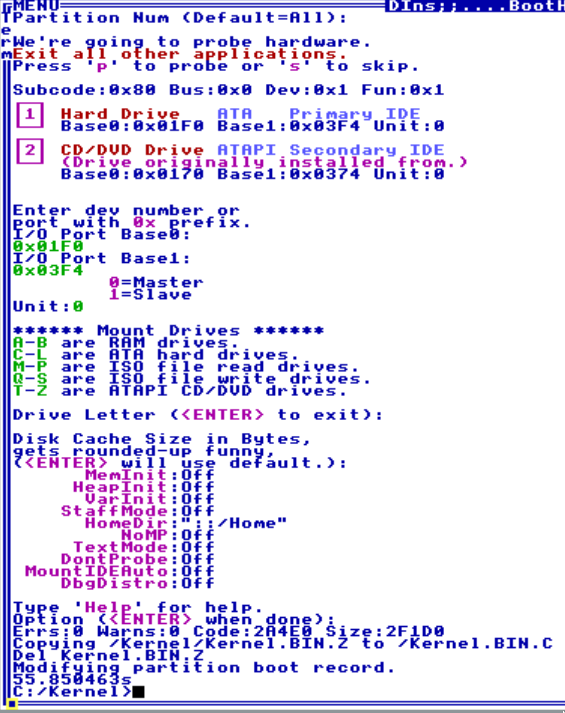
\includegraphics[width=1.0\textwidth]{slike/kernelcomp2.png}
	\caption{Prevođenje jezgre – naprjednije postavke}
    \label{fig:kernelcomp2}
\end{figure}

\chapter{Dodavanje hrvatske tipkovnice u TempleOS}

Praktični zadatak ovoga rada je bio ugraditi hrvatske znakove i tipke u jezgru TempleOS-a, ali je isto tako i dio praktičnoga dijela izraditi usporedbu dodavanja tipkovnice u jezgru s dodavanjem tipkovnice unutar korisničkoga prostora. U sljedećim odjeljcima će se opisati oba procesa, počevši s dodavanjem znakova i tipaka unutar korisničkoga prostora.

\section{Dodavanje u korisnički prostor}

\subsection{Stvaranje vanjskih znakova\label{vanjskiZnakovi}}

Stvaranje vanjskih znakova u TempleOS-u je dosta jednostavno. Uz mali mig iskusnijih programera TempleOS autor je doznao da u kazalu {\fontfamily{pcr}\selectfont /Demo} postoji datoteka koja se zove {\fontfamily{pcr}\selectfont ExtChars.HC.Z}. U toj datoteci je dokumentiran proces izradbe vanjskoga znaka. U primjeru koji je izradio g. Davis se je nalazilo polje {\fontfamily{pcr}\selectfont face} od osam 8-bitnih nepredznačenih cijelih brojeva. Može se opaziti da jedinice u takvu zapisu predstavljaju jedan \emph{pixel}, da zajedno čine smješka, a da su znakovi zapravo bitmape dimenzije 8x8 bitova.

\begin{figure}[H]
    \centering
    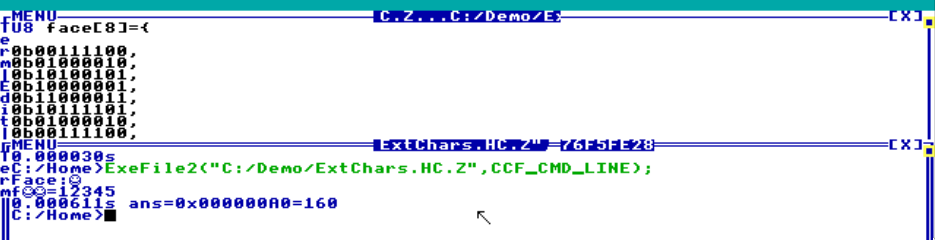
\includegraphics[width=1.0\textwidth]{slike/extchars1.png}
    \caption{Zadani primjer unutar datoteke {\fontfamily{pcr}\selectfont ExtChars.HC.Z}}
    \label{fig:extchars1}
\end{figure}

Ovaj primjer je malo nezgodan jer se na njem ne može opaziti jedan problem koji će se prikazati na Sl. \ref{fig:extchars2}, a to je da je zapis \emph{little-endian}, pa se trebaju izvrnuti bitovi u redcima. U primjeru sa smješkom to se nije vidjelo jer je smješko simetričan po y-osi, pa je u svrhu prikaza izrađen preinačeni primjer koji prikazuje istu stvar, ali na kojem se može opaziti izvrnutost x-osi, a primjer prikazuje hrvatski znak {\fontfamily{pcr}\selectfont Č}.

\begin{figure}[H]
    \centering
    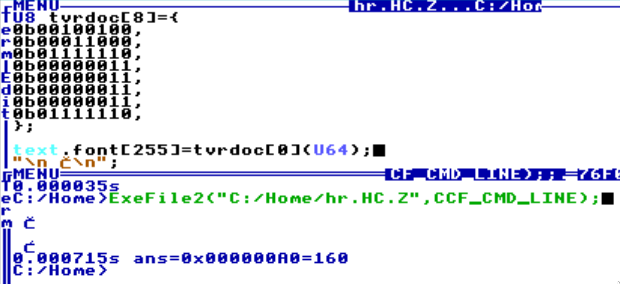
\includegraphics[width=1.0\textwidth]{slike/extchars2.png}
    \caption{Preinačeni primjer vanjskoga znaka}
    \label{fig:extchars2}
\end{figure}

\subsection{Promjena rasporeda tipaka}

Raspored tipaka unutar korisničkog prostora najjednostavnije se može odraditi tako da se izrade svi znakovi postupkom opisanim u odjeljku \ref{vanjskiZnakovi}, da se pohrane u jednu datoteku i da se izvrši {\fontfamily{pcr}\selectfont \#include} te datoteke. Kada se izrade svi potrebni znakovi, potrebno je promijeniti raspored tipaka, da ne bi došlo do zbrke u semantici prigodom izmjenjivanja jezika. Raspored se može odrediti definiranjem dekodne tablice u zbirnom jeziku, koja se ostvaruje jednostavno kao polje 8-bitnih znakova. Preinačene znakove je moguće ubaciti pomoću kombinacije tipaka {\fontfamily{pcr}\selectfont CTRL-ALT-A}, pozicioniranja na željeni znak, i pritiska {\fontfamily{pcr}\selectfont SPACE}-tipke. Nakon izrade dekodnih tablica, rečene je potrebno ubaciti u memoriju, što se radi pomoću funkcije \emph{MemCpy}.

\begin{figure}[H]
    \centering
    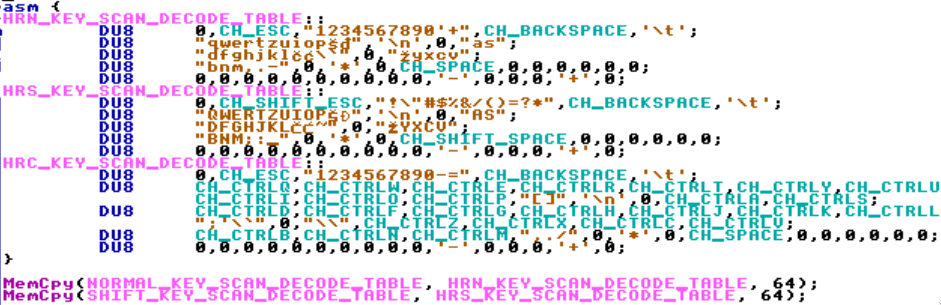
\includegraphics[width=1.0\textwidth]{slike/user_layout.png}
    \caption{Primjer dekodne tablice i njezina učitavanja u memoriju}
    \label{fig:user_layout}
\end{figure}

\section{Dodavanje u jezgru}

\subsection{Stvaranje \emph{fonta} unutar jezgre\label{kreiranjeFontaJezgra}}

Unutar kazala {\fontfamily{pcr}\selectfont /Kernel} mogu se opaziti datoteke {\fontfamily{pcr}\selectfont FontStd.HC.Z} i {\fontfamily{pcr}\selectfont FontCyrilli\-c.HC.Z}. Uz pomoć izvrsne funkcije {\fontfamily{pcr}\selectfont Find} dostupne u TempleOS-u, lako se može otkriti da postoji mogućnost da se u \emph{fontu} dodaju ćirilični znakovi na pritisak tipaka {\fontfamily{pcr}\selectfont CTRL-ALT-F} (QEMU će to zabilježiti kao naredbu za cijeli zaslon i ne će utjecati na TempleOS, pa je stoga potrebno učiniti sljedeće: prisitsnuti {\fontfamily{pcr}\selectfont CTRL-ALT-2}, upisati {\fontfamily{pcr}\selectfont sendkey ctrl-alt-f}, pritisnuti {\fontfamily{pcr}\selectfont CTRL-ALT-1}). Ali prvo se treba opisati proces stvaranja \emph{font}-datoteke , pa se onda baviti dodavanjem novih kombinacija tipaka.

Prvo treba kopirati datoteku {\fontfamily{pcr}\selectfont FontStd.HC.Z} i nazvati ju po želji. Autor ju je nazvao {\fontfamily{pcr}\selectfont FontHr.HC.Z}. Na prvi pogled izgleda kao da se radi o apsolutnim memorijskim adresama gdje su znakovi definirani, iako adrese izgledaju dosta slučajne. Nakon neuspješne potrage gdje su te adrese preslikane, gdje u kodu se definira \emph{font}, i sl., autor se je dosjetio da to uopće nisu adrese, nego da je to heksadekadski prikaz tih znakova, gdje dva znaka predstavljaju jedan bajt.

Ono što se razlikuje od dodavanja u korisničkom prostoru je što su u jezgri osi x i y suprotne od intuitivnoga očekivanja korisnika, dok je kod korisničkoga dodavanja vanjskoga znaka samo x-os izokrenuta (\emph{little endian}). To se najzornije može opaziti na Sl. \ref{fig:fontchar}, gdje se može vidjeti kako je slovo {\fontfamily{pcr}\selectfont Č} zakrenuto za 180°.

\begin{figure}[H]
    \centering
    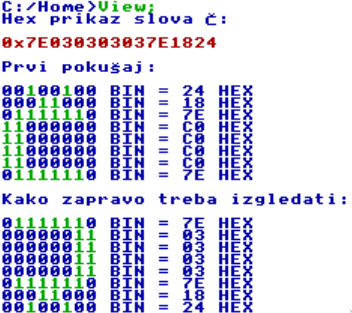
\includegraphics[width=1.0\textwidth]{slike/fontchar.png}
    \caption{Primjer znaka u heksadekadskom zapisu}
    \label{fig:fontchar}
\end{figure}

\subsection{Obavljanje radnjâ na pritisak tipke\label{obavljanjeRadnjiNaPritisak}}

Sljedeći očigledan korak koji se mora ostvariti je obavljanje radnjâ na pritisak tipke, slično kao što se mora pritisnuti kombinacija tipaka da bi se prebacilo na ćirilični \emph{font}. Prvi korak koji se čini je pogled u dokumentaciju, u kazalo {\fontfamily{pcr}\selectfont /Doc} u TempleOS-u. Tu se mogu opaziti dvije datoteke koje počinju s {\fontfamily{pcr}\selectfont Key*}. Iz datoteke {\fontfamily{pcr}\selectfont KeyAlloc.DD.Z} se može opaziti da su kombinacije tipaka {\fontfamily{pcr}\selectfont ALT} i {\fontfamily{pcr}\selectfont ALT-SHIFT} slobodne da ih korisnik dodijeli kako želi, ali da se kombinacija {\fontfamily{pcr}\selectfont CTRL-ALT} obrađuje na sustavskoj razini pomoću funkcije {\fontfamily{pcr}\selectfont CtrlAltCBSet()}. Autor TempleOS-a je uzeo za pravo da predbilježi tipke kako on želi, što je stvaralo sukobljenost u izradbi završnog rada, te je donešena odluka autora da će se rabiti tipka {\fontfamily{pcr}\selectfont ALT} umjesto {\fontfamily{pcr}\selectfont CTRL-ALT}. Tipka {\fontfamily{pcr}\selectfont ALTGR} ima isti \emph{scan code} kao i tipka {\fontfamily{pcr}\selectfont ALT} unutar operacijskoga sustava.

Pomoću funkcije {\fontfamily{pcr}\selectfont Find} se može potražiti funkcija {\fontfamily{pcr}\selectfont CtrlAltCBSet}, gdje se ona rabi, i nakon pretrage da se opaziti da se dosta rabi u datoteci {\fontfamily{pcr}\selectfont /Kernel/KeyDev.HC.Z}.

Funkcije su izvrsno imenovane, stoga se lako da pronaći funkcija koja je odgovorna za izmjenu standardnoga i ćiriličnoga \emph{fonta}, i tu se mogu pronaći korisni tragovi kako dalje s projektnim zadatkom.

Za ispitivanje je dodana kombinacija tipaka {\fontfamily{pcr}\selectfont CTRL-ALT-i} koja bi samo ispisala tekst {\fontfamily{pcr}\selectfont Hello World} na zaslon. Nakon prevođenja jezgre preko funkcije {\fontfamily{pcr}\selectfont BootHDIns;} sve je radilo kao i očekivano. Nakon toga treba kopirati i izmijeniti dio koda odgovoran za izmjenu \emph{fontova} (to je redak {\fontfamily{pcr}\selectfont SwapI64(\&text.font, \&text.font\_hr);}) i alocirati ga za {\fontfamily{pcr}\selectfont CTRL-ALT-p}, te je taj dio za sad gotov, ali poslije će se vratiti na nj u odjeljku \ref{dinamickoIzmjenjivanjeTipkovnice}.

\subsection{Dodavanje \emph{fonta} u memoriju}

Iako je datoteka {\fontfamily{pcr}\selectfont FontHr.HC.Z} u jezgri stvorena, nekako ju je trebalo učitati u samu jezgru da bi se prepoznala u procesu kompilacije AOT jezgre. Važne lokacije za inicijaliziranje \emph{fonta} su vidljive na Sl. \ref{fig:fontloc}.

Koristeći se funkcijom {\fontfamily{pcr}\selectfont Find} mogu se pronaći dva važna mjesta gdje se rabi pokazivač iz funkcije {\fontfamily{pcr}\selectfont SwapI64} iz prethodnoga poglavlja, a to su {\fontfamily{pcr}\selectfont KMain.HC.Z} i {\fontfamily{pcr}\selectfont KernelA.HH.Z}.

U {\fontfamily{pcr}\selectfont KernelA.HH.Z} treba dodati odgovarajući pokazivač na hrvatski \emph{font}, koji čini globalnu varijablu za tekst, a u datoteci {\fontfamily{pcr}\selectfont KMain.HC.Z} toj varijabli treba dodijeliti naziv polja iz naše \emph{font}-datoteke.

Sada se na pritisak tipaka {\fontfamily{pcr}\selectfont CTRL-ALT-p}, kao i iz naredbene ljuske, mogu mijenjati \emph{fontovi}. Budući da je sav tekst u TempleOS-u na engleskom jeziku, vidne promjene nisu opazive na prvi pogled, ali se mogu opaziti tek otvaranjem znakovnoga izbornika na pritisak {\fontfamily{pcr}\selectfont CTRL-ALT-a}.

\begin{figure}[H]
    \centering
    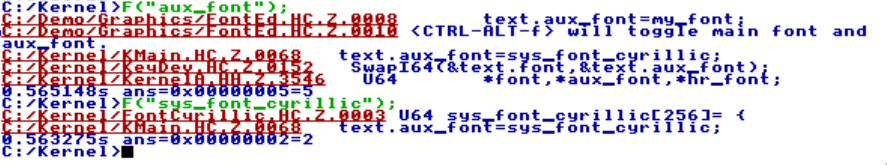
\includegraphics[width=1.0\textwidth]{slike/lokacijeFonta.png}
	\caption{Sve važne lokacije gdje se \emph{font} inicijalizira u memoriji (primjer s ćiriličnim \emph{fontom})}
    \label{fig:fontloc}
\end{figure}

\subsection{Dodavanje novoga rasporeda tipaka}

Izmjena \emph{fonta} nije sama po sebi dovoljna prigodom izradbe tipkovnice. Na primjer, kada bi se imao tekst na engleskom jeziku koji bi glasio {\fontfamily{pcr}\selectfont yes;}, i kada bi se samo izmijenio \emph{font} dobio bi se ozbiljan problem, na hrvatskom bi taj tekst u potpunosti izgubio značenje, glasio bio {\fontfamily{pcr}\selectfont zesč}. To je zbog temeljno drukčijega rasporeda tipaka (eng. \emph{layout}) između tih dviju tipkovnica. U engleskoj tipkovnici {\fontfamily{pcr}\selectfont Z} se nalazi na položaju {\fontfamily{pcr}\selectfont Y}, znak {\fontfamily{pcr}\selectfont ;} se nalazi na položaju slova {\fontfamily{pcr}\selectfont Č}, i sl. Stoga je bilo potrebno locirati datoteku gdje je raspored tipaka definiran, i uz malo kopanja po kazalu {\fontfamily{pcr}\selectfont /Kernel} može se vidjeti da se raspored tipaka nalazi u datoteci {\fontfamily{pcr}\selectfont /Kernel/SerialDev/Keyboard.HC.Z}.

Ispitivanja radi, mogu se izmijeniti položaji slova {\fontfamily{pcr}\selectfont Z} i {\fontfamily{pcr}\selectfont Y}, ponovno prevesti jezgra, i ispitati radi li sve kako treba. Nakon uspješnoga ispitivanja valja vratiti datoteku u izvorno stanje, te ju kopirati u datoteku s nazivom po izboru. Autor je rabio naziv {\fontfamily{pcr}\selectfont KeyHr.HC.Z}. U toj datoteci se dodaju hrvatski znakovi na mjesto gdje pripadaju. Također se treba izraditi i datoteka koja bi služila čisto za izmjenu varijabli. Autor ju je nazvao {\fontfamily{pcr}\selectfont Temp.HC.Z}. Ta datoteka postoji iz razloga kad bi se hrvatsla tipkovnica kopirala u englesku, raspored tipaka engleske tipkovnice se ne bi mogao dobiti natrag. Učinjene izmjene su vidljive na Sl. \ref{fig:layouti}.

\begin{figure}[H]
    \centering
    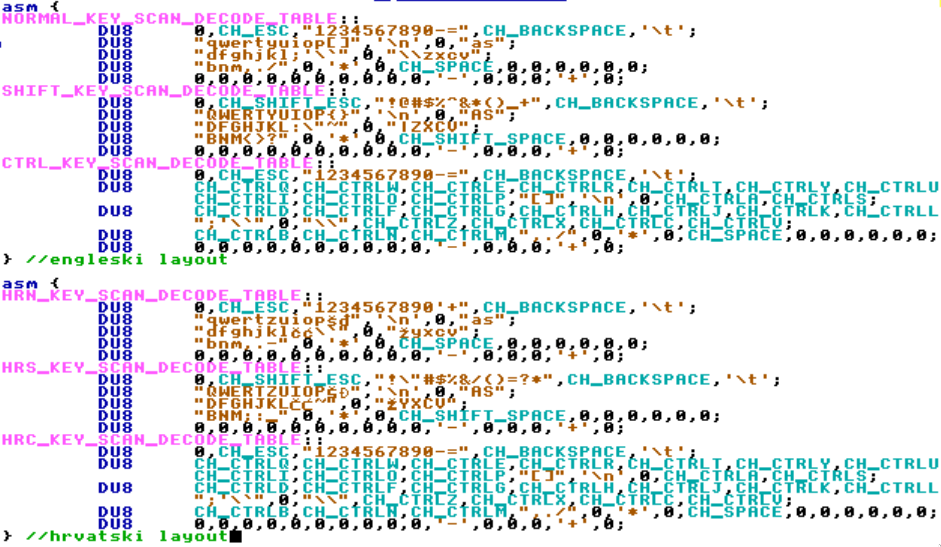
\includegraphics[width=1.0\textwidth]{slike/layouti.png}
	\caption{Usporedba rasporeda tipaka}
    \label{fig:layouti}
\end{figure}

Prevođenje jezgre u trenutačnoj fazi bi davalo pogrješke, jer su funkcije definirane u {\fontfamily{pcr}\selectfont Keyboard.HC.Z} već definirane. Kada bi se pokušale obrisati iz kopirane datoteke, to bi isto tako imalo problema što se tiče dinamičkoga izmjenjivanja tipkovnice. Javio se je problem gdje su vrijednosti iz zbirnoga jezika u navedenim datotekama morale biti prevedene prije datoteke {\fontfamily{pcr}\selectfont KeyDev.HC.Z}, ali jednostavni {\fontfamily{pcr}\selectfont \#include} prije {\fontfamily{pcr}\selectfont KeyDev.HC.Z}-a ne bi radio jer bi funkcije koje se nalaze u datoteci {\fontfamily{pcr}\selectfont Keyboard.HC.Z}-a zahtijevale funkcije iz datoteke {\fontfamily{pcr}\selectfont KeyDev.HC.Z}. Ukratko i pojednostavljeno, A jepotrebno uključiti prije B, a B je potrebno uključiti prije A, što je proturječno. O tome više u poglavlju \ref{dinamickoIzmjenjivanjeTipkovnice}.

\subsection{Dinamičko izmjenjivanje tipkovnice\label{dinamickoIzmjenjivanjeTipkovnice}}

Kada su svi koncepti iznad izrađeni, preostaje još dodati i dinamičko izmjenjivanje tipkovnice, odnosno da se na pritisak kombinacije tipaka izmijene \emph{font} i raspored tipaka.

Proces dodavanja kombinacije {\fontfamily{pcr}\selectfont CTRL-ALT} je opisan u odjeljku \ref{obavljanjeRadnjiNaPritisak}, ali u ovom odjeljku će se potanje obrazložiti što se sve događa unutar kombinacije {\fontfamily{pcr}\selectfont CTRL-ALT-p}, za koju je odlučeno da će biti okidač za dinamičku izmjenu tipkovnica. Dio koda koji se pokrene pri pritisku kombinacije tipaka {\fontfamily{pcr}\selectfont CTRL-ALT-p} će se potanje razmotriti u Sl. \ref{fig:ctrlaltp}.

\begin{figure}[H]
    \centering
    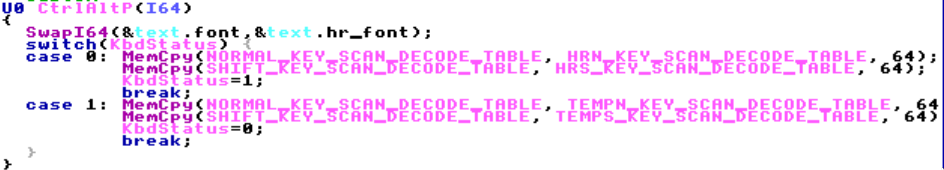
\includegraphics[width=1.0\textwidth]{slike/ctrlaltp.png}
	\caption{Funkcija za dinamičko izmjenjivanje tipkovnice}
    \label{fig:ctrlaltp}
\end{figure}

Funkcija {\fontfamily{pcr}\selectfont SwapI64}, odnosno kako se ista rabi za izmjenu \emph{fonta}, je već opisana u poglavlju \ref{obavljanjeRadnjiNaPritisak}. Ona se obavlja pri svakom pozivu, tako da nije potrebno stavljati ju u {\fontfamily{pcr}\selectfont switch}. {\fontfamily{pcr}\selectfont KbdStatus} je globalna varijabla koja je jednostavno inicijalizirana na ništicu na samom početku datoteke {\fontfamily{pcr}\selectfont KeyDev.HC.Z}, a ona služi za praćenje stanja, da vidi koja je tipkovnica trenutačno djelatna.

Potom se odvija kopiranje jednoga dijela memorije u drugi, odnosno kopira se vrijednost koja je navedena u zbirnom kodu kod definiranja \emph{layouta}. To se obavlja uz pomoć funkcije {\fontfamily{pcr}\selectfont MemCpy}. U programskom jeziku HolyC se ne mogu proslijediti strukture veće od 8 bajtova kao što se mogu u C-u, stoga je odlučeno da će se rabiti {\fontfamily{pcr}\selectfont MemCpy} veličine 64 bajta. Ako se pogleda Sl. \ref{fig:layouti}, može se opaziti da se dio u zbirnom jeziku sastoji od 5 polja 8-bitnih nepredznačenih cijelih brojeva, znači svaki znak se sastoji od jednog bajta. Ručnim brojenjem tih znakova može se doći do zaključka da struktura zauzima između 75 i 80 bajtova, ali isto tako može se opaziti da su zadnji redci isti, te ih nije potrebno kopirati, i tim se je količina podataka za kopiranje smanjila za 16 bajtova.

{\fontfamily{pcr}\selectfont NORMAL\_KEY\_SCAN\_DECODE\_TABLE } obilježava tablicu koja je djelatna, a {\fontfamily{pcr}\selectfont HRN\_KE\-Y\_SCAN\_DECODE\_TABLE } obilježava hrvatsku tipkovnicu ({\fontfamily{pcr}\selectfont HRN} znači {\fontfamily{pcr}\selectfont HR Normal} ). Ista stvar se radi i sa tipkama koje se dobiju uz tipku {\fontfamily{pcr}\selectfont SHIFT}, u {\fontfamily{pcr}\selectfont SHIFT\_KEY\_SCAN\_DECODE\_TABLE} se kopiraju vrijednosti iz {\fontfamily{pcr}\selectfont HRS\_KEY\_SCAN\_DECODE\_TABLE}. {\fontfamily{pcr}\selectfont CTRL\_KEY\_SCAN\_DECODE\_TABLE} n\-ije potrebno kopirati jer su to funkcijske tipke koje su iste za svaki jezik, npr. kombinacija tipaka {\fontfamily{pcr}\selectfont CTRL-B} gasi i pali rubove prozora.

Ovim procesom je izrađena velika većina tipkovnice, ali valja opaziti da još nedostaju {\fontfamily{pcr}\selectfont ALT} tipke, kako bi prikazali znakove poput {\fontfamily{pcr}\selectfont \textbackslash}, {\fontfamily{pcr}\selectfont @}, {\fontfamily{pcr}\selectfont €}, {\fontfamily{pcr}\selectfont <}, {\fontfamily{pcr}\selectfont >}, {\fontfamily{pcr}\selectfont |}, i sl. Više o tom u odjeljku \ref{dodavanjeALTTipaka}.

\subsection{Dodavanje {\fontfamily{pcr}\selectfont ALT}-tipaka \label{dodavanjeALTTipaka}}

Iako se čini kao dosta trivijalan zadatak, dodavanje {\fontfamily{pcr}\selectfont ALT}-tipaka se je pokazalo zahtjevnijim problemom nego što se čini. Naime, prvi pokušaj ostvarivanja kombinacije {\fontfamily{pcr}\selectfont ALT}-tipaka je bio ubacivanje istih u kod zbirnoga jezika koji je definirao i raspored tipaka. Pomoću funkcije {\fontfamily{pcr}\selectfont Find} da se opaziti da su konstante definirane u zbirnom jeziku automatski dostupne u svim dijelovima jezgre, kao što je i već viđeno u datoteci {\fontfamily{pcr}\selectfont KeyDev.HC.Z}. Drugo spominjanje tih konstantata se je spominjalo u datoteci s tipkovničnim funkcijama koje su već ranije u radu logički odvojene od zbirnoga koda, a to je {\fontfamily{pcr}\selectfont Keyboard1.HC.Z}. Nakon dosta pokusâ s tom datotekom, odnosno s {\fontfamily{pcr}\selectfont ScanCode2Char } funkcijom (kao i s funkcijom {\fontfamily{pcr}\selectfont Char2ScanCode}), iz nekoga razloga jednostavno nije radilo, pa je odlučeno da će se tražiti alternativno rješenje.

Alternativno rješenje je bilo uzeti datoteku {\fontfamily{pcr}\selectfont HomeKeyPlugIns.HC.Z}, koja se nalazi u korijenskom kazalu TempleOS-a, te ju staviti u Adam, te ju {\fontfamily{pcr}\selectfont \#include}-ati prigodom paljenja operacijskoga sustava. Budući da je Adam prvi proces koji se stvara i ne može se ugasiti, on se može smatrati sustavskim dijelom operacijskoga sustava. Jedina razlika je što se on obavlja kompilacijom Just In Time, za razliku od jezgre, koja je jedini dio sustava koja se prevodi Ahead Of Time.

U datoteci {\fontfamily{pcr}\selectfont /Doc/KeyDev.HC.Z} je opisano kako se pomoću funkcije {\fontfamily{pcr}\selectfont KeyDevAdd} dodaju nove funkcionalnosti za tipkovnicu, a za svrhe ovog rada najbolje bi bilo rabiti korisnički rukovatelj {\fontfamily{pcr}\selectfont MyPutKey} jer je on od svih opisanih rukovatelja najprikladniji za operacije potrebne za izradbu ciljanog zadatka. Na Sl. \ref{fig:altTipke1} i \ref{fig:altTipke2} je prikazan proces dodavanja tih tipaka, dok je proces dodavanja \emph{fonta} već opisan u poglavlju \ref{kreiranjeFontaJezgra}.

Kod vidljiv na Sl. \ref{fig:altTipke1} je sam po sebi jasan. Prvi uvjet \emph{if} govori da tipka {\fontfamily{pcr}\selectfont ALT} mora biti pritisnuta, te da tipka {\fontfamily{pcr}\selectfont CTRL} ne smije biti pritisnuta. {\fontfamily{pcr}\selectfont CTRL} uvjet služi samo zato da ne bi bilo nekih konfliktnih kombinacija koje bi obavljale dvije radnje u isto vrijeme, kao npr. u slučaju kombinacije {\fontfamily{pcr}\selectfont CTRL-B}, gdje bi se napisao znak {\fontfamily{pcr}\selectfont \{}, ali bi se i uklonile granice prozora TempleOS-a. Ostatak se svodi na to da ovisno o tom koji znak TempleOS primi, i ako taj \emph{scan code} nema opis u sustavu, da stavi neki drugi znak.

Na Sl. \ref{fig:altTipke2} postoji jedan dio koda koji nije jasan na prvi pogled, pa ga valja objasniti. To je uvjet koji glasi {\fontfamily{pcr}\selectfont if(sc\&0x7F==0x56)}. Razlog zašto se obavlja logičko I se nalazi u datoteci {\fontfamily{pcr}\selectfont /Doc/CharOverview.HC.Z}. U datoteci se može opaziti opis povratne vrijednosti pritisnute tipke, odnosno da ništični bajt sadržava \emph{scan code}, te da bi se on dohvatio potrebno je se nekako riješiti zastavice ispred, a to se može obaviti pomoću trunkacije viših bajtova, koja se može odraditi bitovnim I. Budući da se na tipkovnici rabe ASCII znakovi od 0 do 127, može se rabiti heksadekadski broj {\fontfamily{pcr}\selectfont 7F}, jer on kad se zapiše binarno sadržava 7 jedinica, tako da će se sve iznad toga truncirati. Nije pogrješka rabiti heksadekadski broj {\fontfamily{pcr}\selectfont FF}, jer ASCII u TempleOS-u je 8-bitni, ali budući da se na tipkovnici samo nalaze znakovi od 0 do 127, dok se znakovima s višim vrijednostima može pristupiti samo pomoću kombinacije tipaka {\fontfamily{pcr}\selectfont CTRL-ALT-a}.

Razlog zašto se rabi {\fontfamily{pcr}\selectfont 0x56} je što je to \emph{scan code} tipke kojom se pišu znakovi {\fontfamily{pcr}\selectfont <}, {\fontfamily{pcr}\selectfont >} i {\fontfamily{pcr}\selectfont |}. Njezin \emph{scan code} se može doznati preko datoteke {\fontfamily{pcr}\selectfont MsgLoop.HC.Z} koja se nalazi u kazalu {\fontfamily{pcr}\selectfont /Demo}.

Dodavanjem te tipke je pokrivena cijela tipkovnica. Funkcijom {\fontfamily{pcr}\selectfont KeyDevAdd} se dodaju izrađene tipke {\fontfamily{pcr}\selectfont ALT}, te je još nužno obaviti {\fontfamily{pcr}\selectfont \#include} naše datoteke u datoteci {\fontfamily{pcr}\selectfont MakeAdam.HC.Z} u kazalu {\fontfamily{pcr}\selectfont /Adam}, i tim je projektni zadatak gotov.

\begin{figure}[H]
    \centering
    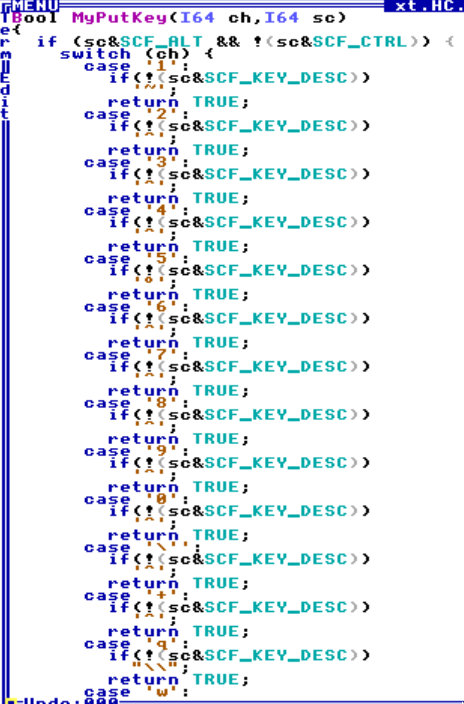
\includegraphics[width=1.0\textwidth]{slike/altTipke1.png}
	\caption{Funkcija {\fontfamily{pcr}\selectfont MyPutKey} u kojoj se definira ponašanje tipkovnice}
    \label{fig:altTipke1}
\end{figure}

\begin{figure}[H]
    \centering
    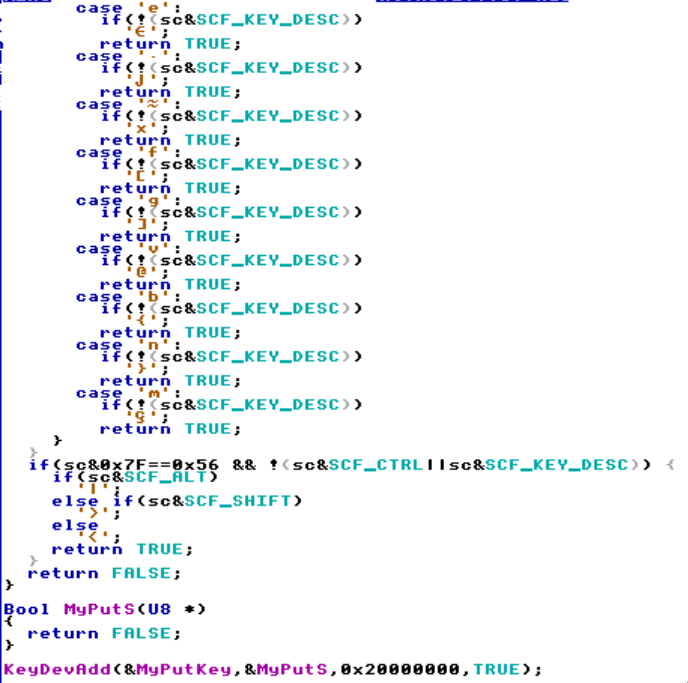
\includegraphics[width=1.0\textwidth]{slike/altTipke2.png}
	\captionsetup{justification=centering}
	\caption{Ostatak funkcije {\fontfamily{pcr}\selectfont MyPutKey} i funkcija {\fontfamily{pcr}\selectfont KeyDevAdd} gdje se dodaje funkcija {\fontfamily{pcr}\selectfont MyPutKey} kao tipkovnični uređaj}
    \label{fig:altTipke2}
\end{figure}

\chapter{Prevođenje, pokretanje i ispitivanje sustava}

U posljednjem poglavlju završnoga rada se obrađuje proces prevođenja i pokretanja izmjenjene inačice TempleOS sustava.

\section{Prevođenje preinačenoga TempleOS-a\label{dodavanjeALTTipaka}}

Kada je cijela tipkovnica napravljena, postavlja se pitanje kako se napravljeno može podijeliti s drugima. Jedan izbor bi svakako bio podijeliti sliku virtualnoga stroja s drugima, ali to bi zauzimalo onoliko koliko je autor sam odredio prostora, u ovom slučaju 3 gigabajta, što je masivno i nepraktično za dijeljenje.

Bolji izbor je rabiti program {\fontfamily{pcr}\selectfont DoDistro.HC.Z} koji je dostupan u samom TempleOS-u, pod kazalom {\fontfamily{pcr}\selectfont /Misc}. {\fontfamily{pcr}\selectfont \#include}-anjem te datoteke se kopira sve što se nalazi u operacijskom sustavu, pa čak i rječnik, koji opcionalno može obrisati da bi se uštedjelo na prostoru (ovom primjeru je uključen i rječnik, te je ukupna veličina ISO-datoteke 31 MB). Nakon što se stvori ISO-datoteka, može se locirati u kazalu {\fontfamily{pcr}\selectfont /Tmp}.

Kada je stvorena vlastita distribucija, postavlja se pitanje kako ISO-datoteku koja se nalazi unutar TempleOS-a prenijeti izvan operacijskoga sustava, budući da TempleOS ne podupire mrežne operacije. Nakon malo pokusiranja, pa zatim istraživanja, pronađena su dva načina, ovisno o vrsti diska koja se ima, je li to obličje \emph{raw} ili \emph{qcow2} \cite{QEMUArchWiki}.

Ako se ima obličje slike \emph{raw}, naredba koja se pokreće jest:

\begin{lstlisting}[language=sh,caption={Montiranje obličja slike \emph{raw}},captionpos=b]
#!/bin/sh
# montiranje
sudo mount -o loop,offset=32256 staza/do/slike staza/montiranja
\end{lstlisting}

Ako se pak radi o obličju slike \emph{qcow2}, naredbe koje se pokreću su:

\begin{lstlisting}[language=sh,caption={Montiranje obličja slike \emph{qcow2}},captionpos=b]
#!/bin/sh
# montiranje
sudo modprobe nbd max_part=16
sudo qemu-nbd -c /dev/nbd0 staza/do/slike
sudo partprobe /dev/nbd0
sudo mount /dev/nbd0p1 staza/montiranja
\end{lstlisting}

Nakon tog postupka korisniku su dostupne sve datoteke iz operacijskoga sustava TempleOS, te je samo potrebno prekopirati ISO-datoteku distribucije iz staze montiranja na željenu stazu izvan staze montiranja, te obvezno odmontirati montiranu sliku, inače će vrlo vjerojatno doći do gubitka podataka!

\begin{lstlisting}[language=sh,caption={Odmontiranje obličja slike \emph{raw}},captionpos=b]
#!/bin/sh
# odmontiranje
sudo umount staza/montiranja
\end{lstlisting}

\begin{lstlisting}[language=sh,caption={Odmontiranje obličja slike \emph{qcow2}},captionpos=b]
#!/bin/sh
# odmontiranje
sudo umount staza/montiranja
sudo qemu-nbd -d /dev/nbd0
sudo partprobe
\end{lstlisting}

\section{Pokretanje preinačenoga TempleOS-a}

Proces instalacije je identičan procesu opisanom u poglavlju \ref{instalacijaTOSa}, osim što umjesto službene ISO-slike skida se preinačena slika, dostupna na \url{https://viktoracoric.xyz/files/TOSHR.ISO.C}.

U svrhu ovoga rada će se rabiti virtualni stroj QEMU, iako bi procedura na drugim virtualnim strojevima kao npr. VirtualBox i VMWare trebala biti dosta čak i jednostavnija.

Prvo je potrebno stvoriti sliku virtualnoga diska. Za to se rabi sljedeća naredba:

\begin{lstlisting}[language=sh,caption={Stvaranje virtualnoga diska},captionpos=b]
# stvaranje diska (velicina je opcionalna, velicina u megabajtima se izrazava u brojevima bez slova G)
qemu-img create -f qcow2 ~/tos.qcow2 2G
\end{lstlisting}

Nakon što je virtualni disk stvoren, treba pokrenuti virtualni stroj.

\begin{lstlisting}[language=sh,caption={Pokretanje virtualnoga stroja QEMU u svrhu instalacije putem naredbenoga redka},captionpos=b]
qemu-x86_64 -enable-kvm -cpu host -soundhw pcspk -drive file=tos.qcow2 -cdrom TOSHR.ISO.C -m 2G
\end{lstlisting}

Argumenti iz naredbe za pokretanje u svrhu instalacije obilježavaju sljedeće:

\begin{itemize}
    \item {\fontfamily{pcr}\selectfont -enable-kvm} znači da se rabi modul Kernel-based Virtual Machine, koji omogućuje sklopovsku virtualizaciju.

    \item {\fontfamily{pcr}\selectfont -soundhw pcspk} je opcionalni argument koji nam omogućuje zvuk unutar TempleOS-a.

    \item {\fontfamily{pcr}\selectfont -cpu host} izbor daje najprecizniju emulaciju za procesor koji korisnik posjeduje.

    \item {\fontfamily{pcr}\selectfont -drive file=[staza]} pruža željenu datoteku virtualnoga diska.

    \item {\fontfamily{pcr}\selectfont -cdrom [staza]} pruža instalacijsku datoteku rabeći pogon CD-ROM.

    \item {\fontfamily{pcr}\selectfont -m [broj]} specificira koliko će radne memorije virtualni stroj rabiti. Potrebno je dati minimalno 512 MB.
\end{itemize}

Nakon toga slijedi već opisani proces instalacije, koji je sam po sebi jasan, ali ako nije može se podsjetiti u posljednjem odlomku poglavlja \ref{instalacijaTOSa}. Operacijski sustav se pokreće sljedećom naredbom:

\begin{lstlisting}[language=sh,caption={Pokretanje virtualnoga stroja QEMU preko naredbenoga retka},captionpos=b]
qemu-x86_64 -enable-kvm -cpu host -soundhw pcspk -drive file=tos.qcow2 -m 2G
\end{lstlisting}

\section{Ispitivanje preinačenoga TempleOS-a}

Nakon što instalacija završi, novoinstalirani operacijski sustav TempleOS se može ugasiti, a iz naredbe iznad se može izbaciti argument {\fontfamily{pcr}\selectfont -cdrom}. U novoinstaliranom operacijskom sustavu se može ispitati već iznad opisani proces kojim je hrvatska tipkovnica dodana u sustav: pritisnuti {\fontfamily{pcr}\selectfont CTRL-ALT-p} za promjenu tipkovnice na hrvatski jezik, ispitati sve tipke, te po potrebi prebaciti natrag na englesku tipkovnicu.

Model prikazan na Sl. \ref{fig:crokeyboardlayout} će poslužiti kao referentni model za ispitivanje, jer je hrvatska tipkovnica za TempleOS i rađena po prikazanom modelu.

\begin{figure}[H]
    \centering
    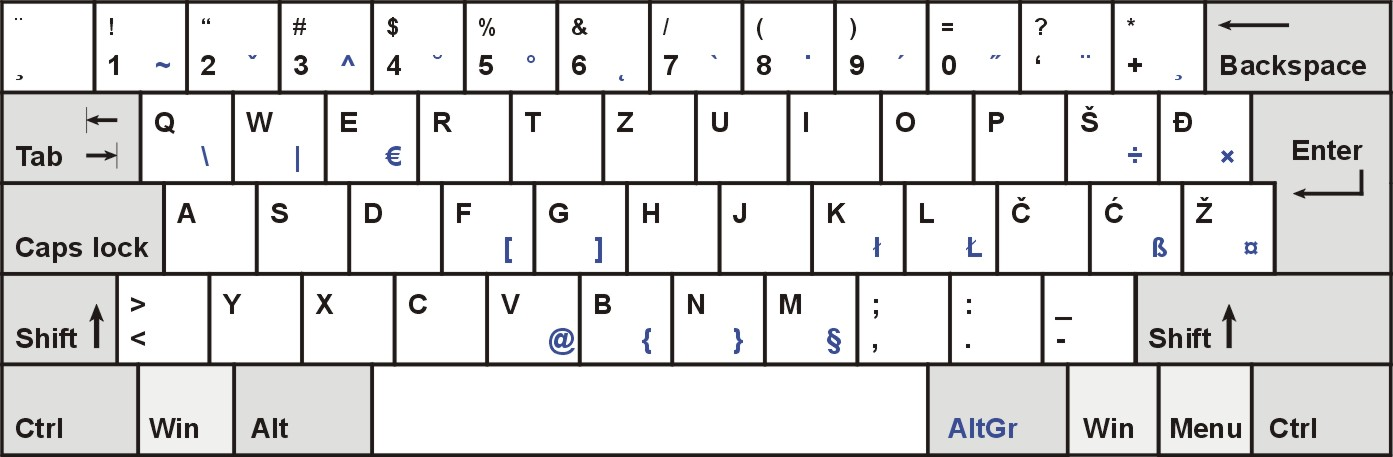
\includegraphics[width=1.0\textwidth]{slike/crokeyboardlayout.jpg}
	\captionsetup{justification=centering}
	\caption{Referentni model hrvatske tipkovnice}
    \label{fig:crokeyboardlayout}
\end{figure}

Ispitivanje se vrši pritiskanjem tipaka, ispituju se tipke bez ikakva kombiniranja, tipke u kombinaciji s tipkom {\fontfamily{pcr}\selectfont SHIFT}, tipke u kombinaciji s tipkom {\fontfamily{pcr}\selectfont ALT}, te tipke u kombinaciji s tipkom {\fontfamily{pcr}\selectfont ALT}. Tipke u kombinaciji s tipkom {\fontfamily{pcr}\selectfont CTRL} su iste kao i na zadanoj engleskoj tipkovnici, te ih stoga nije nužno ispitati. U radu je već objašnjeno zašto se ne rabe tipke u kombinaciji s tipkama {\fontfamily{pcr}\selectfont CTRL} i {\fontfamily{pcr}\selectfont ALT}, razlog je taj što operacijski sustav TempleOS već rabi neke funkcije na mjestu gdje bi se inače rabili određeni znakovi.

Kada se završi s ispitivanjem, postoji mogućnost i vratiti se na englesku tipkovnicu ako korisnik to želi.

\chapter{Zaključak}

Nakon završene preinake operacijskoga sustava TempleOS, valja se osvrnuti na učinjeno, na sam proces izradbe, na prednosti i nedostatke pristupa opisanih u radu, te prokomentirati procese i metode koje su se ostvarivale u svrhu postizanja cilja.

Instalacija TempleOS-a unutar virtualnoga stroja je prilično jednostavna i cijeli proces je automatiziran. U radu je demonstrirano da se cijeli operacijski sustav instalira za minutu, i to samo uz par pritisaka na tipkovnici. TempleOS nudi i vodič oko sustava, što može puno pomoći korisniku što se tiče osnovne porabe, no za naprjedniju porabu operacijskoga sustava ipak treba imati predznanje iz programiranja. Programski jezik HolyC je vrlo jednostavan za porabu, ali je ujedno i moćan programski jezik koji nudi jednostavan rad s grafikama, dovoljno je jednostavan za podučavanje predškolske djece o programiranju, ali i dovoljno naprjedan da se može isprogramirati TCP/IP stog i pružiti potpora za mrežne operacije. Iz toga se može naslutiti da je dodavanje funkcionalnosti u korisnički prostor, kao i u jezgru, dosta pristupačno, te složenost dodavanja funkcionalnosti ovisi o samoj složenosti te funkcionalnosti.

U radu su se obradila dva načina dodavanja hrvatske tipkovnice, dodavanje unutar korisničkoga prostora i unutar korisničke jezgre. Oba pristupa imaju svoje prednosti i nedostatke. Dodavanje tipkovnice unutar korisničkoga prostora teorijski može biti fleksibilnije, jer iako nije učinjeno u ovom radu, može se ostvariti da se jedan jezik stavi u jednu datoteku. Nedostatak ovoga pristupa je nemogućnost dinamičkoga izmjenjivanja tipkovnice, za koje bi bilo potrebno proširiti jezgru, a bez takve proširke bi trebalo dosta više vremena za obavljanje tako jednostavne operacije. Još jedan nedostatak pristupa dodavanjem unutar korisničkoga prostora jest težina izradbe samog \emph{fonta}. Prednost dodavanja u jezgru operacijskoga sustava je ta što se tipkovnice mogu izmjenjivati dinamički na pritisak tipke. Nedostatak je što kad bi se uključivalo više tipkovnica unutar operacijskoga sustava, operacijski sustav bi rastao u veličini, što je očigledno nešto što je suprotno onomu što je autor TempleOS-a zamislio, budući da je se često hvalio činjenicom da njegov operacijski sustav zauzima svega 2 MB. Još jedan nedostatak je to što je uključivanje fonta i rasporeda tipaka nešto teže.

Također se vrijedi i osvrnuti na metode distribucije učinjenoga unutar operacijskoga sustava TempleOS. U radu je rabljena distribucija cijeloga operacijskog sustava, ali isto tako se može napraviti i instalacijski program koji bi kopirao preinačene datoteke na svoje mjesto. Između ovih dvaju pristupa nema nekih prednosti i nedostataka osim veličine ISO-datoteke, ali se je autor odlučio za prvi pristup jer on ne zahtijeva nikakvo međudjelovanje s korisnikom prigodom prevođenja i pokretanja preinačene inačice operacijskog sustava, dok bi drugi način zahtijevao prevođenje jezgre, koje se vrši Ahead Of Time (AOT), koje zahtijeva korisničku interakciju.

Bilo kako bilo, ovaj rad je pokazao da se potpora za različite tipkovnice može izraditi uz malo truda. Iako je proces dosta jednostavan kada se opiše u radu, proces izradbe je naporniji dio, ali je i iznimno zanimljiv i prigodom izradbe se nauči dosta novih stvari.

\printbibliography[title=Popis literature]
\addcontentsline{toc}{chapter}{Popis literature}

\listoffigures
\addcontentsline{toc}{chapter}{Popis slika}

%\listoftables
%\addcontentsline{toc}{chapter}{Popis tablica}

%\lstlistoflistings
%\addcontentsline{toc}{chapter}{\lstlistlistingname}

%\appendix
%\renewcommand{\thechapter}{\arabic{chapter}}

%\chapter{Prilog 1}

%\chapter{Prilog 2}

\end{document}

{\fontfamily{pcr}\selectfont }
